\chapter{High-Level Architecture}

Calico's new architecture was motivated by the design decisions listed below. 
The key design decisions for the new version of Calico were:

\begin{itemize}\itemsep1pt
  \item Client/Server architecture for improved connectivity over the Internet.
  \item Optimization of network traffic to reduce lag on distant clients, as well as network usage.
  \item A plugin framework to enable developers to create extensions into the Calico system.
  \item Improvement of input event handling system to improve drawing performance and input recognition.
  \item Consistency handling and persistence improvements to ensure that clients are all kept in the same state.
\end{itemize}

In the following sections, each decision will be explained in more detail.



\section{Client/Server Architecture}
We decided that the architecture needed to be redesigned in order to support all the planned changes. The new architecture that was chosen had to be able to support all the features, as well as easily support multiple users simultaneously. It also had to be accessible from anywhere, and had to be more stable than previous versions that were known to crash.

\begin{figure}[h]
\centering
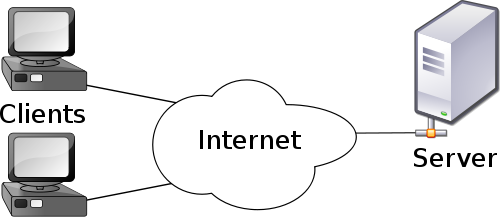
\includegraphics[width=0.8\textwidth]{fake_arch.png}
\caption{Overview of Calico's Architecture}
\label{fig:calico_arch}
\end{figure}

The first change made was a switch from the original peer-to-peer system to a completely new client-server architecture. We believed that by using a client-server architecture, we could provide a centrally accessible service that would easily support multiple clients and still maintain stability. The server could act as a headless service that could be more efficient since it did not have to perform any client functions such as rendering the display. This meant that the server could be dedicated to the task of managing all the interactions between clients, and could be much more stable than in a peer-to-peer context. When using peer-to-peer, each client was responsible for notifying all connected clients (which caused a large amount of network traffic). By switching to client-server, clients are only communicating with a single server, which greatly reduced the network traffic, and increased the stability of the network.

\section{Networking Component Overhaul}
One of the significant changes from the original Calico was the change in network communication design. The previous version of Calico had networking that was designed as an add-on at a later time, and was not fully integrated into the system. In this old design, when a change was made by another client, the entire change was saved to a Java object. This object was then serialized and sent in full over the network. The receiving client would deserialize this data, and then perform the change on its local drawing canvas. This process was very easy to implement, but had the cost of requiring significant processor time due to the constant serialization/deserialization process that would take place for each action. It also incurred the network overhead of Java serialization, which would add much more data to the final packet. All of this overhead would quickly become apparent to users when the system would lag in response to many actions done in quick succession. Our goal was to streamline this process as much as possible so that we could reduce lag when the system was being heavily utilized.

To improve the responsiveness of Calico, and reduce the network overhead, we created a custom packet design that could be used by Calico to notify both the client and server when various actions were performed. These special packets provided exactly what was needed to effectively communicate changes to clients, and thereby significantly reduced in size compared to the original design. Packets now are byte arrays that are written directly to the wire and, based on the format expected by the given command, are decoded back into their specific components (integers, strings, booleans, and floats). 



\begin{figure}[h!]
  \centering
  \begin{bytefield}{34}
    \bitbox{4}{length} & \bitbox{8}{command ID} & \bitbox{24}{command-specific data}
  \end{bytefield}
  \caption{A Calico network packet}
\label{fig:calico_packet}
\end{figure}

This packet design was loosely based on the packet design of the Half-Life game engine \cite{rcon}. As seen in the figure above, the packet is broken up into three main parts. The first four bytes of the packet is the length of the packet. This tells the network system how much farther it needs to read to ensure it receives the entire packet. The next four bytes hold the command identifier. This number is used to tell the network system what this packet is about. Both the client and the server have a list of commands and their IDs, which are used to translate from a programmer-friendly command name to the command ID number. The remaining bytes vary based on the specific command that is being transmitted. Each command has different parameters, of which both the client and server are aware. By writing data directly to the wire, there is little overhead -- each packet is as small as it could be. This makes the network communication between the client and server much more efficient, and helps to reduce the lag, even when put under heavy usage.

\section{Improvement of Input Handling System}
In the previous version of Calico, the input system was plagued by sluggish performance and inaccuracy. When there were many elements on the screen, the input system would lag and would begin to ``miss'' input data, which would result in straight lines instead of smooth curves. As a sketching tool, the ability to receive accurate input from the user was very important to the performance of the tool. The previous version of Calico routed input data directly to the rendering system, which would draw the images on screen. This made development very easy, but it required the input system to wait on the rendering process. This meant that the more images that had to be rendered, the longer the input system had to wait before it could start processing new input data. In Java, the mouse input listener does not queue input events -- if a program is too busy to receive input, then that input event is lost forever. Due to this problem, fluid drawing was nearly impossible.   

The new version of Calico is designed to fix this problem. By creating a separate, but dedicated input handling system, Calico can readily process input commands without having to wait for the rendering process to complete.

Instead of linking the input, action processing, and rendering systems serially, they are now linked in ``parallel'' using a multi-threaded approach. None of the separate processes are reliant on any of the other processes to complete, so input can be quickly received and queued if needed. These input events are then sent to the action processing system which determines what actions (if any) should be performed based upon the given input. Once an action is decided, the rendering process is notified and redraws the screen as needed. By using these components in parallel, we are able to remove the perceived lag and missed mouse events that would cause distortion and incorrect sketching. Even though the display can lag slightly behind the rendering system, this delay is not nearly as noticeable as when input events were being missed. 


\section{Consistency Handling / Persistence}
The previous version of Calico had many problems maintaining consistency between all clients. Clients would quickly become outdated and their states would not be consistent with that of the other clients. 
This problem was generally a result of parallel edits being performed. Clients would perform the edits locally, and then notify the other clients of the change. Often, the events would be received in a different order than they were being performed on a client, and the elements would be modified incorrectly. This led to identical elements being displayed very differently on multiple clients, due to the fact that there was no authority to resolve disputes when edits were being done to an element at the same time.
The previous version of Calico had no central server to check or update consistency, so any time where a client became inconsistent, designers had to quit the program and reconnect in order to fix the problem.
Naturally, this was very frustrating to users as it made it very difficult to collaborate with another user once the data became inconsistent. 

In the new version of Calico, this problem is fixed by implementing a system for checking and maintaining consistency across all clients connected to the server. In the new Calico, the server is considered to be the master, and all clients defer to the server to determine what state they should be at. All client actions are sent to the server and are not processed on the client until the server acknowledges the command. This means that all clients are given the same commands to modify elements at the same time. Clients are essentially ``unintelligent'' and do not assume any knowledge of where elements should be positioned -- this is all maintained by the server. This means that clients never become inconsistent, as there is a single system that is responsible for maintaining the state on each client system. 
Even when clients are editing the same element in parallel, Calico is able to maintain consistency by giving priority to the first event received. This allows users to edit the same element, and prevents the system from trying to issue conflicting edits to the same object.

The only time when clients now lose consistency was during network errors where packet loss is experienced. However, even if this were to occur, there are regular consistency checks that quickly realize the inconsistencies and fix them, without ever interrupting the designer. This system periodically notifies all clients of the current state of the system by sending a hash code to all clients. The hash code represents a checksum of the system and all of the drawing content. If any of the clients responds with a different hash code, they are sent an export of the entire session containing all the data needed to recreate the canvas from scratch. Because of this, any inconsistencies could easily be mitigated with minimal inconvenience to the end user. This meant that a session using the new version of Calico could last for weeks without problem -- something that was not possible in the previous version of Calico. The only drawback with this new process is that sometimes content changes unexpectedly for the user when parallel changes or packet loss occurs. While this is disruptive, the frequency of this occurring is low.
